\section{Usability}\label{usability}
Ins Deutsche übersetzt bedeutet Usability nach \citeauthor{usability} (\citeyear{usability}) Gebrauchstauglichkeit oder Nutzerfreundlichkeit.
Sie sorgt dafür, dass Programme einfach verwendet werden können.
Gemessen wird sie daran, wie schnell und direkt ein Benutzer sein Ziel während der Nutzung der Software erreicht.
Die Norm DIN EN ISO 9241 beschreibt einige Eigenschaften, welche eine Anwendung mit hoher Usability haben soll.
Diese sind:
\begin{itemize}
   \item der Aufgabe angemessen
   \item selbst beschreibend
   \item steuerbar
   \item erwartungskonform
   \item fehlertolerant
   \item lernförderlich
   \item motivierend
\end{itemize}
Um diese Eigenschaften zu erreichen, ist ein entsprechendes Vorgehen während der Entwicklung nötig.
Dies wir im nächsten Abschnitt erläutert.


\subsection{Projektablauf mit Usability als Ziel}
\citeauthor{usability} (\citeyear{usability}) sagen, dass die Nutzer während der Entwicklung möglichst früh eingebunden werden.
So kann von ihnen die Bestätigung eingeholt werden, dass das Entwickelte gefällt.
Wenn es nicht gefällt, so kann wieder von vorne angefangen werden.
Laut \citeauthor{usability} ist in einem optimalen Projektablauf der Nutzer in jeder Phase eingebunden.
So soll in einer ersten Phase der Nutzer kennengelernt und verstanden werden.
Dazu werden im folgenden Abschnitt einige Methoden erklärt.
In einer nächsten Phase sollen die Anforderungen der Nutzer spezifiziert werden.
Diese sollen in der dritten Phase anhand von Prototypen umgesetzt und in der letzten Phase von den Nutzern evaluiert werden.
Agile Vorgehensmodelle eignen sich gut, um regelmässig Tests mit den Nutzern durchzuführen, beispielsweise nach jedem Sprint.
Die vier erwähnten Phase können wiederholt durchgeführt werden.
Um in der vierten Phase möglichst positive Testergebnisse zu erhalten, gibt es Richtlinien, welche befolgt werden können.
Auf diese wird in Abschnitt \ref{guidelines} genauer eingegangen.


\subsection{Methoden um die Nutzer kennen zu lernen}
Um Anforderungen an die Anwendung formulieren zu können, sollen zuerst die Nutzer dieser Anwendung kennengelernt und deren Bedürfnisse sowie Wünsche erfasst werden.
\citeauthor{usability} (\citeyear{usability}) nennen dazu mehrere Methoden.
Diese werden hier vorgestellt:

\subsubsection{Fokusgruppen}\label{fokusgruppe}
Bei einer Fokusgruppe handelt es sich um eine Gruppendiskussion.
Ein Moderator führt mit fünf bis zehn Personen ein Gespräche zu einem bestimmten Thema.
So können bestehende Anwendungen verbessert oder Ideen für neue gesammelt werden.
Ein erstelltes Konzept kann den Nutzern erstmals gezeigt und von ihnen evaluiert werden.
Der Austausch innerhalb der Fokusgruppe soll gefördert werden, da dies die Kreativität anregt.
Es kann hilfreich sein, wenn sich die Teilnehmer der Diskussion im Voraus auf diese vorbereiten.
So sind sie gezwungen, bereits vor der Diskussion eine Meinung zu bilden und es kann vermieden werden, dass sich Teilnehmer der Gruppenmeinung anschliessen.


\subsubsection{Befragungen}\label{befragung}
Ziel einer Befragung ist es, die individuellen Meinungen von Einzelpersonen zu erfassen.
In der Regel werden sie mithilfe eines Fragebogens durchgeführt.
Im Gegensatz zu den Fokusgruppen sind sie eher dazu da, um quantitative Daten zu erheben und weniger für die Erfassung neuer Ideen geeignet.
Wird dieselbe Befragung über längere Zeit mehrmals durchgeführt, können Veränderungen oder Trends gemessen werden.


\subsubsection{Vor-Ort-Beobachtungen}\label{vorort}
Bei einer Vor-Ort-Beobachtung wird der Benutzer aus dem Hintergrund bei einer typischen Nutzungssituation beobachtet.
Er soll dabei vom Beobachter möglichst wenig beeinflusst werden, so dass seine Abläufe möglichst alltäglich sind.
Der Beobachter notiert, wie die Software verwendet wird.
Dabei soll speziell auf unbewusstes Verhalten der Nutzer geachtet werden.


\subsubsection{Tagebuchstudien}\label{tagebuchstudien}
Bei Tagebuchstudien erfassen die Nutzer ihr eigenes Verhalten.
Entweder bei der Nutzung einer konkreten Anwendung oder in Situationen bei denen eine geplante Anwendung eingesetzt werden soll.
So können Erlebnisse der Nutzer über einen längeren Zeitraum gesammelt werden.
Ereignisse und Erfahrungen welche unregelmässig oder gar einmalig auftreten, können so erfasst werden.
Dies ist bei Vor-Ort-Beobachtungen nur schwer möglich.

\subsection{Usability Guidelines}\label{guidelines}
Bewährte Guidelines können befolgt werden, um eine hohe Usability zu erreichen.
\citeauthor{usability} (\citeyear{usability}) kennen Guidelines zu unterschiedlichen Aspekten einer Anwendungen.
Einige dieser Aspekte und die zugehörigen Guidelines werden in den folgenden Abschnitten erläutert.

\subsubsection{Informations- und Navigationsarchitektur}
Die Informations- und Navigationsarchitektur bildet das Fundament einer Anwendung.
Während sie bei kleineren Anwendungen noch vernachlässigt werden kann, so muss sie bei grösseren Anwendungen ausführlich geplant werden.
Das Ziel einer guten Informations- und Navigationsarchitektur ist, dass ein Nutzer schnell und einfach zu den gewünschten Informationen navigieren kann.
Dies kann erreicht werden, indem die Inhalte zuerst grob sortiert werden.
Diese Sortierung wird dann als Grundlage genommen, um eine feine Gliederung zu erarbeiten.
Dabei ist wichtig, dass nicht ein perfektes, logisches System das Ziel ist, sondern eine Architektur, welche für den Nutzer intuitiv zu bedienen ist.


\subsubsection{Gestaltungsraster}
Gestaltungsraster sind dazu da, um die Elemente einer Benutzeroberfläche geordnet darzustellen.
Im Gestaltungsraster wird die Seite oder das Fenster mittels Führungslinien in Reihen und Spalten eingeteilt.
Diese Linien geben an, wo Elemente platziert werden können und wie viel Abstand zwischen ihnen ist.
In Abbildung \ref{fig:Gestaltungsraster} sind mehrere solcher Raster aufgezeigt.
\begin{figure}[H]
   \centering
   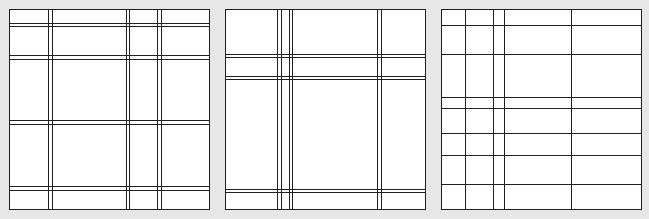
\includegraphics[width=1.0\textwidth]{gfx/Gestaltungsraster_aus_buch.png}
   \caption{
      Verschiedene Gestaltungsraster welche mittels Führungslinien unterteilt sind.
   }
   \source{\citeauthor{usability}}
   \label{fig:Gestaltungsraster}
\end{figure}
Bereits die ersten Entwürfe der Benutzerschnittstelle sollen auf ein Raster gezeichnet werden.
Bei der Programmierung der Benutzerschnittstelle können diese Einteilungen direkt übernommen werden.


\subsubsection{Farben}
Farben sind für die Gestaltung von Benutzerschnittstellen sehr wichtig.
Ansprechende Anwendungen machen bei der Nutzung Freude und hinterlassen einen positiven Eindruck.
Die Auswahl von Farben und was als ästhetisch wahrgenommen wird, ist subjektiv.
Trotzdem gibt es einige Richtlinien, welche befolgt werden können:
\begin{itemize}
   \item Bestimmte Farben werden oft der gleichen Eigenschaft zugeordnet. So bedeutet Grün of \dq In Ordnung\dq, während Rot oft mit \dq Gefahr\dq in Verbindung gebracht wird. Solche Eigenschaften sollen gezielt eingesetzt werden.
   \item Wichtige Elemente einer Anwendungen können mit auffälligen Farben hervorgehen werden.
   \item Bei Anwendungen, welche über längere Zeit verwendet werden, sollen Farben sparsam eingesetzt werden, da diese Ablenken können.
   \item Der Kontrast zwischen Vorder- und Hintergrund soll gross genug sein, damit beispielsweise Text auch bei erschwerten Bedingungen wie Sonnenschein gelesen werden kann.
   \item Um zwei unterschiedliche Elemente zu unterscheiden, sollte nicht einzig auf unterschiedliche Farben gesetzt werden. Menschen tun sich schwer damit, Farben zu unterscheiden.
Für Personen mit einer Rot-Grün-Schwäche ist es teilweise gar unmöglich.
\end{itemize}


\subsubsection{Icons}
Icons bieten die Möglichkeit, platzsparend Auskunft über die Funktion eines Elements wie z.B. einem Knopf zu geben.
Ästhetisch bieten Icons eine ansprechende Abwechslung zu Text.
Gängige Icons wurden von den Benutzern bereits gelernt und kommen ihnen vertraut vor.
Trotzdem sollten Icons wenn möglich mit einem Label beschriftet werden, damit allen Benutzern klar ist, was passiert, wenn z.B. auf einen Knopf geklickt wird.
Die Icons sollen dabei jeweils oberhalb oder rechts vom Label platziert werden, so dass sie im Lesefluss jeweils zuerst wahrgenommen werden.

\subsubsection{Labels}
Labels dienen dazu, um den Nutzern mitzuteilen, was ein Element macht.
Bei Knöpfen sind die Labels jeweils Teil des Knopfs.
Eine beste Position für die Anordnung von Labels bei Eingabefelder gibt es nicht.
So kann das Label beispielsweise oberhalb oder neben dem Eingabefeld angebracht werden oder innerhalb als Platzhalter.
Labels als Platzhalter sind sehr platzsparend, haben jedoch den Nachteil, dass sie nur solange angezeigt werden, bis der Nutzer mit dem Befüllen des Eingabefeld beginnt.
Bei der Wahl der Position eines Labels sollte also beachtet werden, wann und wie lange das Label für den Nutzer sichtbar sein muss.

\subsubsection{Fehlermeldungen}
Fehlermeldungen sollten möglichst früh angezeigt werden.
Gibt der Nutzer beispielsweise ein unerlaubtes Zeichen in ein Eingabefeld ein, so soll er darauf hingewiesen werden, noch bevor er das ganze Formular abschickt oder eine weitere Aktion ausgeführt.
Fehlermeldungen sollten wenn möglich dort angezeigt werden, wo der Fehler verursacht wurde.
Bei der Formulierung der Meldung ist darauf zu achten, dass sie für jeden Nutzer verständlich ist und möglichst spezifisch darauf hinweist, was falsch gemacht wurde.

\subsubsection{Designsysteme}
Nutzer erwarten, dass eine neue Anwendungen gleich funktioniert wie jene, die sie zuvor verwendet haben und bereits kennen.
Um dies zu gewährleisten, kann einem Designsystem gefolgt werden.
Diese enthalten Standards zum Aussehen und der Funktionalität von Benutzerschnittstellen.
Es ist nicht nötig, ein eigenes Designsystem zu entwickeln.
Für unterschiedliche Plattformen und Anwendungszwecke existieren bereits diverse.
In Abbildung \ref{fig:fluent} ist das \textit{Fluent Design System} von Microsoft dargestellt.
Dieses kann unter anderem für die Entwicklung von Windows Desktop Applikationen als Standard verwendet werden.
\begin{figure}[H]
   \centering
   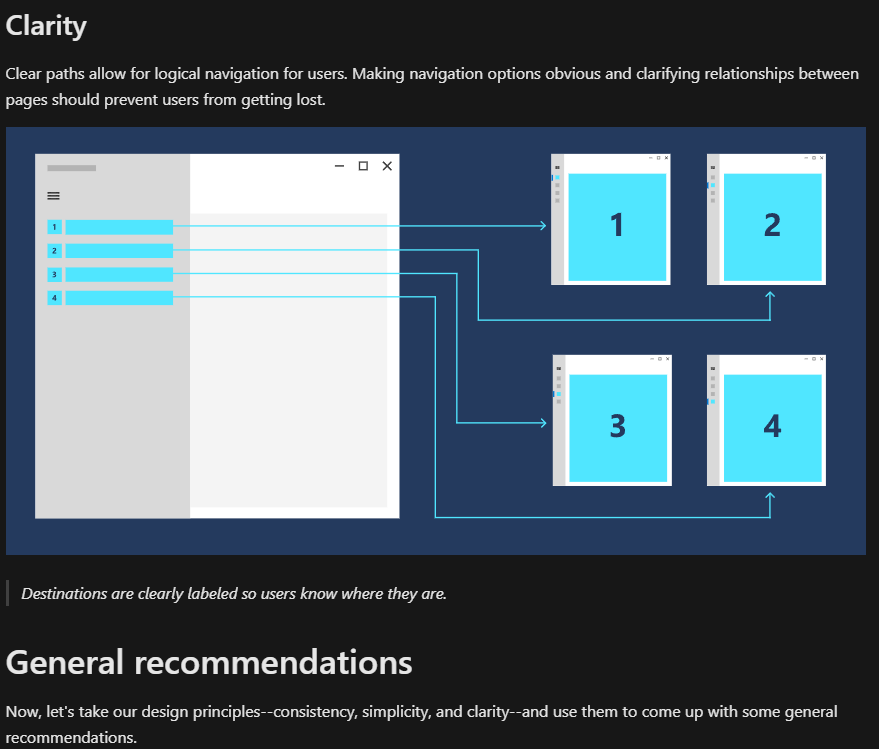
\includegraphics[width=1.0\textwidth]{gfx/design_system_ms.png}
   \caption{
      Ausschnitt aus der Dokumentation zum \textit{Fluent Design System}
   }
   \source{Microsoft}
   \label{fig:fluent}
\end{figure}